\documentclass{beamer}


\usepackage[utf8]{inputenc}
\usepackage{amsmath}
\usepackage{amsfonts}
\usepackage{amssymb}
\usepackage{graphicx}
\usepackage{ragged2e}  % `\justifying` text
\usepackage{booktabs}  % Tables
\usepackage{tabularx}
\usepackage{tikz}      % Diagrams
\usetikzlibrary{calc, shapes, backgrounds}
\usepackage{amsmath}
\usepackage{amssymb}
\usepackage{dsfont}
\usepackage{url}       % `\url
\usepackage{listings}  % Code listings
\usepackage[T1]{fontenc}


\usepackage{theme/beamerthemehbrs}

\author[A. Ortega]{Argentina Ortega S\'ainz}
\title{Introduction to Public Speaking}
\subtitle{Tips and Tricks for MAS}

\institute[HBRS]{Hochschule Bonn-Rhein-Sieg}
% \date{\today}
% \subject{Test beamer}

\begin{document}
{
\begin{frame}
\titlepage
\end{frame}
}

\AtBeginSection[]{% Print an outline at the beginning of sections
\begin{frame}<beamer>
	% \frametitle{Outline for Section \thesection}
	\tableofcontents[currentsection]
\end{frame}%
}%

\section{What to say}

\begin{frame}[t]{What to say}
    \begin{itemize}
        \item \textbf{Think about your audience}
        \begin{itemize}
            \item How much of the basics should you cover?
        \end{itemize}
        \item What is the message of your talk?
        \item \textbf{Start with an outline!}
    \end{itemize}
\end{frame}
%--- Next Frame ---%


\section{What to put in your slides}
\begin{frame}[t]{Content}
    \begin{itemize}
        \item The content of your slides should:
        \begin{itemize}
            \item be self explanatory
            \item use footnotes for new terminology
            \item used to "remind" you of the key points in your speech
        \end{itemize}
        \item Use examples to drive your message
        \item Tell a story
    \end{itemize}
\end{frame}
%--- Next Frame ---%

\begin{frame}[t]{Bullets}
    \begin{itemize}
        \item Avoid filling your slide with a wall of text
        \begin{itemize}
            \item A bullet is a single key point
            \item Indent ideas which are secondary
            \item Only indent bullets which are related to the top level one
        \end{itemize}
        \item About 4-6 bullets per slide is a good measure
    \end{itemize}
\end{frame}
%--- Next Frame ---%
\begin{frame}[t]{Formatting}
    \begin{itemize}
        \item Limit the number of slides (1 slide = 3 minutes aprox)
        \item Font size for your text should be around 24 points
        \item Use contrasting colors, e.g. black fonts on a white background
        \begin{itemize}
            \item You can search for: Color contrast checker
        \end{itemize}
    \end{itemize}
\end{frame}
%--- Next Frame ---%
\begin{frame}[t]{Visual aids}
\vspace{-15pt}
\begin{figure}
    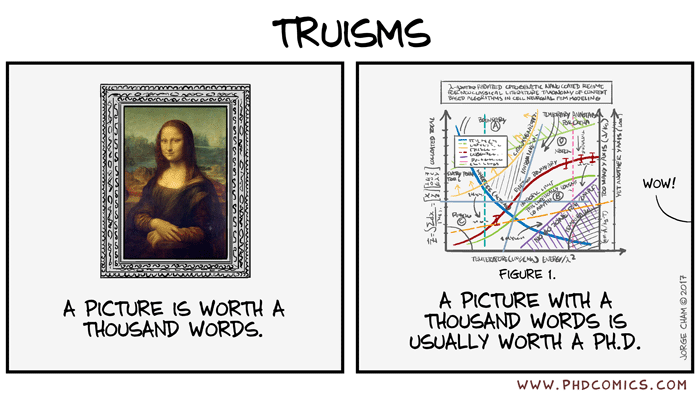
\includegraphics[width=\textwidth]{images/phd022417s}
    \caption{An image is worth a thousand words.\footnote{http://phdcomics.com/comics.php?f=1926}}
    \label{fig:visual-aids}
\end{figure}

\end{frame}
%--- Next Frame ---%
\section{Presenting}

\begin{frame}[t]{Preparations}
    \begin{itemize}
        \item Rehearsing is the most important thing
        \item Don't memorize the text! The information on your slides is an aid for your audience
    \end{itemize}
\end{frame}
%--- Next Frame ---%
\begin{frame}[t]{Giving your talk}
    \begin{itemize}
        \item Breathe!
        \item Modulate your voice
        \item Look at your audience
        \item Use non-verbal queues
    \end{itemize}
\end{frame}
%--- Next Frame ---%

\begin{frame}[t]{Assignments}
    \begin{itemize}
        \item This will be your most common oportunity for practice!
        \item Avoid reading from the assignment, try explaining instead
    \end{itemize}
\end{frame}
%--- Next Frame ---%

\end{document}
